%!TEX root = ../../csuthesis_main.tex
\chapter{深度强化学习理论基础}

\section{强化学习模型}

可观察到强化学习于研究领域内,其亦被称作提高学习或者再励学习,强化学习算法的研究主要聚焦于审视代理同环境之间的交互,于此过程中,代理人挑选环境所提供的有关自身行为的信息,代理依据环境给出的行为信息做出决策并实现更好的学习,这乃是代理与环境间最为关键的交互。其本质为代理与环境交互以生成动作并施行策略,选择这些行动及方法的依据是代理借助环境数据评估系统的状态与性能,强化学习算法无需针对问题构建模型或者熟悉环境,最关键的是数据研究,以此保障代理和环境之间有更佳的互动,优质的数据可使代理的行动与方法得以优化及改进。在激励培训的情形下,理解代理与理解人的学习过程颇为相似,代理依靠与环境的交互获取恰当的奖励,随后借助整合上述奖励与惩罚,代理可得到合适的奖励,经由反复尝试以及持续学习,代理可逐步寻得最为适宜的表现方式,达成全局最优,这种试错学习的进程让代理可逐步提升其于特定环境中的表现以及适应能力。
\subsection{马尔科夫决策过程}


\begin{figure}[hbt]
	\centering
	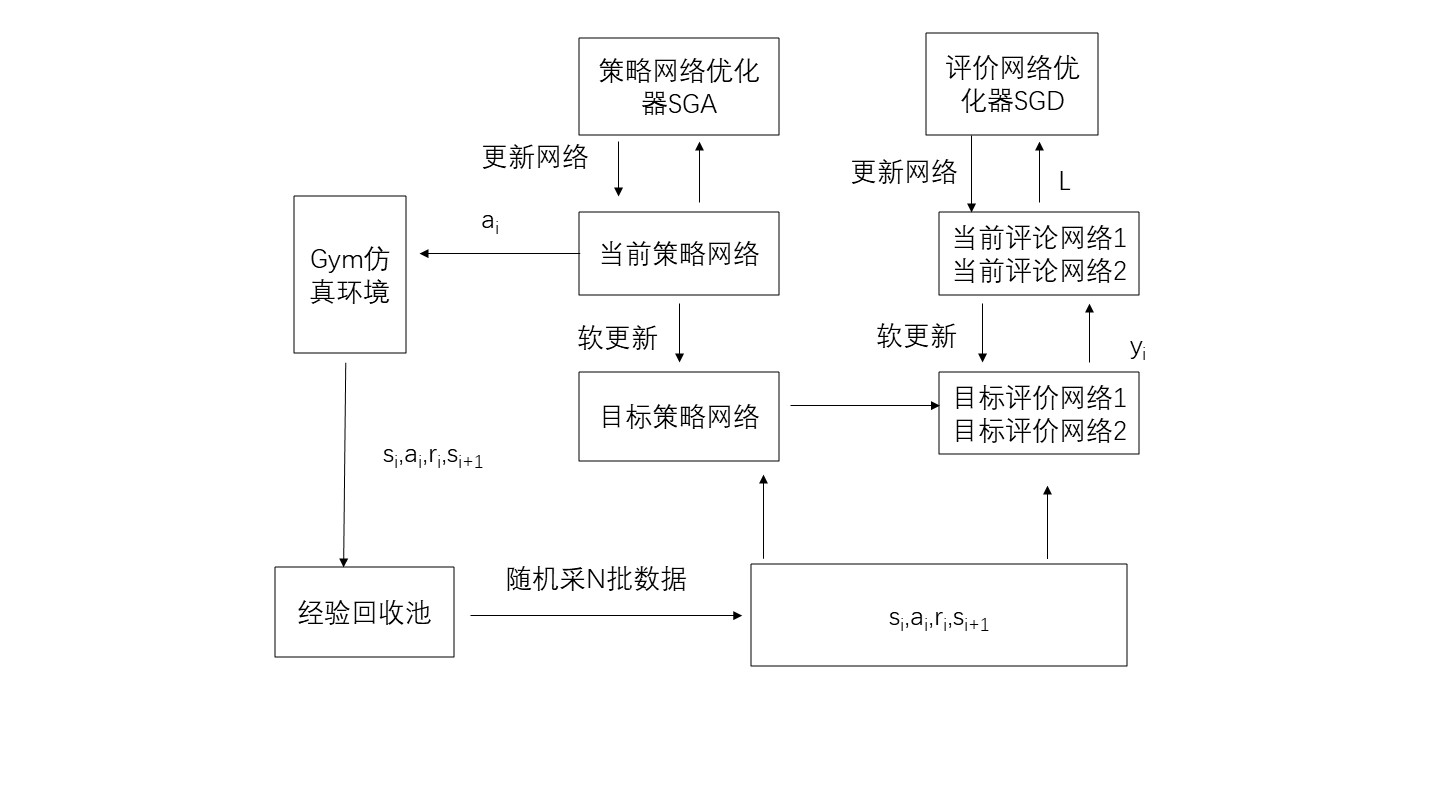
\includegraphics[width=\linewidth]{基于MDP的强化学习结构.jpeg}
	\caption{基于MDP的强化学习结构}
	\label{f.example}
\end{figure}

如果一个系统的状态信息中包含了大量的历史信息,并且不需要提供任何信息,就可以通过结合当前状态来推断出未来的状态,那么这样的状态特性通常被称为马尔可夫特性。结合前面提到的代理与环境的紧耦合,本质上环境的状态是与当前动作紧密相关的,与情境紧密相关的。根据强化学习问题,可以创建马尔可夫决策过程(MDP)\cite{garcia2013markov}。详细流程如上图2-1所示。

智能体获取状态信息,把上述信息当成是输入,结合上述信息,科学选择动作,完成输出。结合动作结果得到相应的奖励,进一步得到未来动作。所以,结合马尔科夫决策过程<$S,A,P,R,$r>
对这一过程进行界定与表述。

首先,需要定义状态。状态是代理接收到的信息,它会对其下一步行动的选择产生一定的影响。状态集群$S$={${s_{1}}$,${s_{2}}$,...,${s_{t}}$}可以由一个或多个动态层组成,通常处理传感器检测到的信息。动作空间$A$={${a_{1}}$,${a_{2}}$,...,${a_{t}}$}表示代理可以选择的动作集合,即它在当前动作中可以选择的所有动作。转移概率表示从当前状态到下一个状态的动作的可能性。如果满足马尔可夫条件,转移概率可以表示为:

\[
P(s_{t+1} \mid s_t, a_t) = P(s_{t+1} \mid s_t, a_t, s_{t-1}, a_{t-1}, \ldots)
\]

可观察到奖励函数属于特定的标量函数,其代表在给定状态下运用环境动作后所获取的回报值,奖励函数依据状态信息展开设计,对代理算法参数的评估以及优化产生影响,折扣因子即折现率,用于对影响当前与未来回报的因素加以加权,可对未来影响因素给予全面分析。

\begin{figure}[hbt]
	\centering
	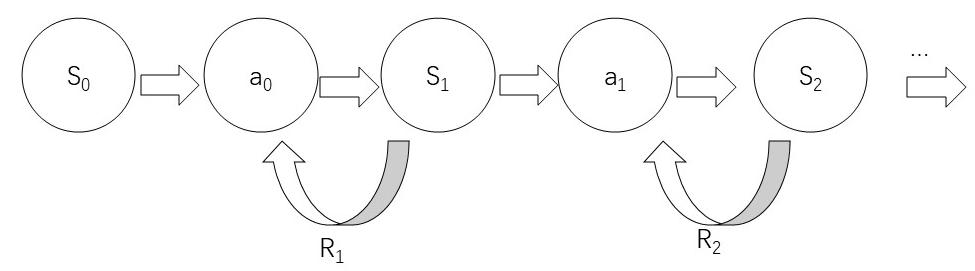
\includegraphics[width=\linewidth]{马尔可夫动态过程.jpeg}
	\caption{马尔可夫动态过程}
	\label{f.example}
\end{figure}

我们可观察到,MDP动态传输方案呈现在上图2-2中,提供者依据当前状态的相关信息作出选择操作,随后把操作反馈给环境,环境作出响应,营造出新的情形并给出有价值的回报,随着代理持续与环境展开交互,并且不断进行学习,直至抵达最终阶段,在我们的领域中察觉到,代理与环境相互作用以施行最优策略并使总奖励实现最大化。MDP的关键概念之一是折扣率,它体现未来收益的折现值,也就是在两个不同时刻状态下未来利润的价值差异,然而MDP通信模型一般基于一个隐含假定,即代理可完全获取所有可用信息,不过在实际情形下,比如针对自动驾驶决策,智能代理借助传感器监测环境,它无法获得完整信息且无法运用MDP假设。当代理观察环境时,其有可能被环境中的其他因素分散注意力,故而接收到的信息仅仅是实际环境信息的一部分。

本篇文章假设转移概率收敛于马尔可夫过程,未来状态仅取决于当前状态与所采取的行动,并非过去状态,不过在高级场景里,传感器提供的信息有限,这意味着我们无法获取无限的状态信息,由此可发现,从状态空间到存储单元存在多种遍历方式,致使存储难以契合马尔可夫链的条件。为解决该问题,研究人员提出了几种方法,比如Shani\cite{shani2013survey}等人开发了一个全面的马尔可夫过程,用于解释代理和环境之间产生的所有相互信息,假设最初的观察和行动契合马尔可夫特性。

\begin{figure}[hbt]
	\centering
	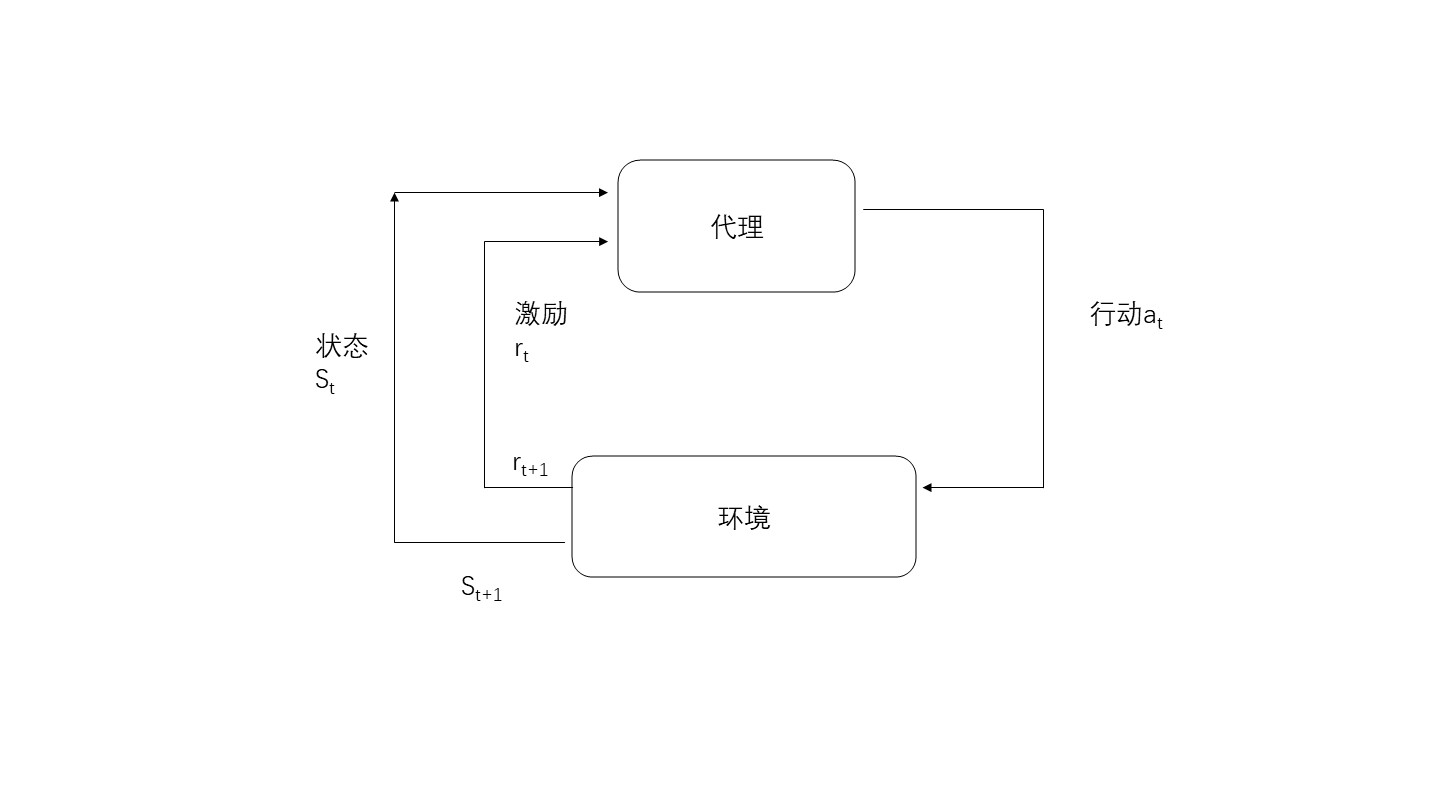
\includegraphics[width=\linewidth]{基于POMMDP的强化学习结构.jpeg}
	\caption{基于POMMDP的强化学习结构}
	\label{f.example}
\end{figure}

上图2-3给出的是环境同代理交互循环关系,收到观察结果以后代理通过采取动作,同环境之间迭代交互,但代理并非了解真实状态信息。

\subsection{价值函数与策略}


可观察到,强化学习存在两个基本构成部分,即财务绩效与策略,这二者于算法的设计以及优化进程里均发挥着关键作用,虽说奖励的当前数值可给出关于当下事态的信息,然而其仅仅反映即时奖励,无法全然预测当前决策的未来结果,若要权衡一个行动的利弊,就要考量其后果,在强化学习算法当中,成本函数是用于明确给定情形下奖励的预期值的关键参数。这一理念一般以两个函数的形式得以实现,分别是交易价值函数以及状态价值函数,状态价值函数一般被用于表示从当前状态至结束状态的期望奖励值,而交易价值函数所描述的是执行某项任务后从当前状态至结束状态的奖励的期望值,借助这两个部分,操作员可更为深入地剖析环境中的各类物体及行为。

可发现,依据交易价值函数以及状态价值函数,可认为状态V的值对于代理从当前状态至最终状态所获取的平均工资存在直接影响,当代理进行决策时,其会倾向于挑选可带来更多价值的方案,借此找到最佳的奖励平衡,改进成本函数后,算法在决策过程中会变得更智能且高效,提升生产力以及加快项目完成速度。

当给定某一状态之时,便会相应地生成与之相关的策略约束,而且可运用独立策略去挑选所有点的约束动作,在给定的特定场景当中,用户会依据任意概率分布来挑选最佳选项,强化学习的目标在于寻得可让所有人的利润实现最大化的最优解,具体呈现如下式子所示:

\[
G_t = R(s_t, a_t) + \gamma R(s_{t+1}, a_{t+1}) + \gamma^2 R(s_{t+2}, a_{t+2}) + \ldots + \gamma^k R(s_{t+k+1}, a_{t+k+1})
\]
\[
= \sum_{k=0}^\infty \gamma^k R(s_{t+k+1}, a_{t+k+1})
\]

\subsection{贝尔曼方程}

为了改进学习数据,状态值和交换率函数是贝尔曼方程的解,可以将其分解为各种问题,并可以作为方程获得良好的解\cite{franccois2018introduction}。计算采用两点,旨在达到理想的平衡。

(1) 贝尔曼期望方程

\[
V_{\pi}(s) = E_{\pi} \left[ G_{t+1} \mid s_{t} = s \right]
\]
\[
= \mathbb{E}_x \left[ R_{t+1}(s_t, a_t) + \gamma R_{t+2}(s_{t+1}, a_{t+1}) + \gamma^2 R_{t+3}(s_{t+2}, a_{t+2}) + \ldots \ \middle| \ s_t = s \right]
\]
\[
= \mathbb{E}_{\pi} \left[ R_{t+1}(s_t, a_t) + \gamma \left( R_{t+2}(s_{t+1}, a_{t+1}) + \gamma R_{t+3}(s_{t+2}, a_{t+2}) + \ldots \right) \ \middle| \ s_t = s \right]
\]
\[
= \mathbb{E}_{\pi} \left[ R_{t+1}(s_t, a_t) + \gamma G_{t+1} \ \middle| \ s_t = s \right]
\]
\[
= \mathbb{E}_{\pi} \left[ R_{t+1}(s_t, a_t) + \gamma V(s_{t+1}) \ \middle| \ s_t = s \right]
\]

根据上述公式,对${V}$进行分解处理以后:当前环境下的立即回报值和下一时刻状态值函数可以被我们清晰的看到。

继续进行同样分解${Q}$,可以得到下式:
\begin{align*}
	\underline{Q}_\pi(s) &= \underline{E} \Big[ G_{t+1} \ \Big| \ S_t = s, A_t = a \Big] \\
	&= \underline{E} \Big[ R_{t+1}(s_t, a_t) + \gamma \underline{Q}_\pi(s_{t+1}) \ \Big| \ S_t = s, A_t = a \Big]
\end{align*}

上述表达式中,由于策略$\pi$的影响,可以计算出所有可能性的对应状态值函数的值的为
Q值与$\pi$的乘积的和。如下式所示:

\[
V_{\pi}(s) = \sum_{a \in A} \pi(a|s) Q_{\pi}(s,a) = \mathbb{E}_{a \sim \pi(a|s)} \left[ Q_{\pi}(s,a) \right]
\]

类似的还有下式:

\[
\underline{O}_{\pi}(s, a) = R(s, a) + \gamma \sum_{s' \in S} p(s' \mid s, a) V_{\pi}(s')
\]

(2) 贝尔曼最优方程

此方程是针对两大值函数的内在联系的全面表述,目的是从中挑选出策略对应的最大值
函数,即为最优值函数$V^*(s)$:

\[
V^*(s) = \arg\max_{\pi} V_{\pi}(s), \quad s \in S
\]

同理可得到,最优动作值函数$Q^*(s,a)$:

\[
Q^*(s, a) = \arg\max_{\pi} Q_{\pi}(s, a), \quad s \in S
\]

依据上述两式可得到$V^*(s)$和$Q^*(s,a)$的直接关系式:

\[
V^*(s) = \arg\max_{a} Q^*(s, a)
\]
\[
Q^*(s, a) = R(s, a) + \gamma \sum_{s' \in S} p(s' \mid s, a) V^*(s')
\]

在离散情况下,设置强化学习任务是以有限状态集为依托的,能够获取不同状态s对应
的$V(s)$函数,或$(s,a)$对应的$Q(s,a)$函数。通过计算出$V(s)$,实施更新迭代,结合策略,确定值函数,进而进行评估。再结合上述式子便可以推导出下列式子:

\begin{align*}
	V_{\pi}(s) &= \sum_{a \in A} \pi(a \mid s) Q_{\pi}(s, a) \\
	&= \sum_{a \in A} \pi(a \mid s) \left( R(s, a) + \gamma \sum_{s' \in S} P(s' \mid s, a) V_{\pi}(s') \right)
\end{align*}

针对MDP问题,求出值函数,获取最佳控制策略,必定能够得到最优策略。想要获取
最大策略$\pi^*$,利用最大的$Q^*(s,a)$函数,可以获取最优策略:

\begin{align*}
	\pi^*(a \mid s) &= \arg\max_{a \in A} Q^*(s, a) \\
	&= \arg\max_{a \in A} \left( R(s, a) + \gamma \sum_{s' \in S} p(s' \mid s, a) V^*(s') \right)
\end{align*}

\section{深度神经网络}

经研究发现,神经网络里深度神经网络系统是复杂多层系统,此多层系统中诸多节点有多个神经元,借助连接权重传输及处理信息,图2 - 4展示了典型深度神经网络架构,其由几个隐藏层与一个输出层构成,每个隐藏层和派生层皆含若干节点,每个节点和前一层所有节点相连,且有一定权重与偏移量。

\begin{figure}[hbt]
	\centering
	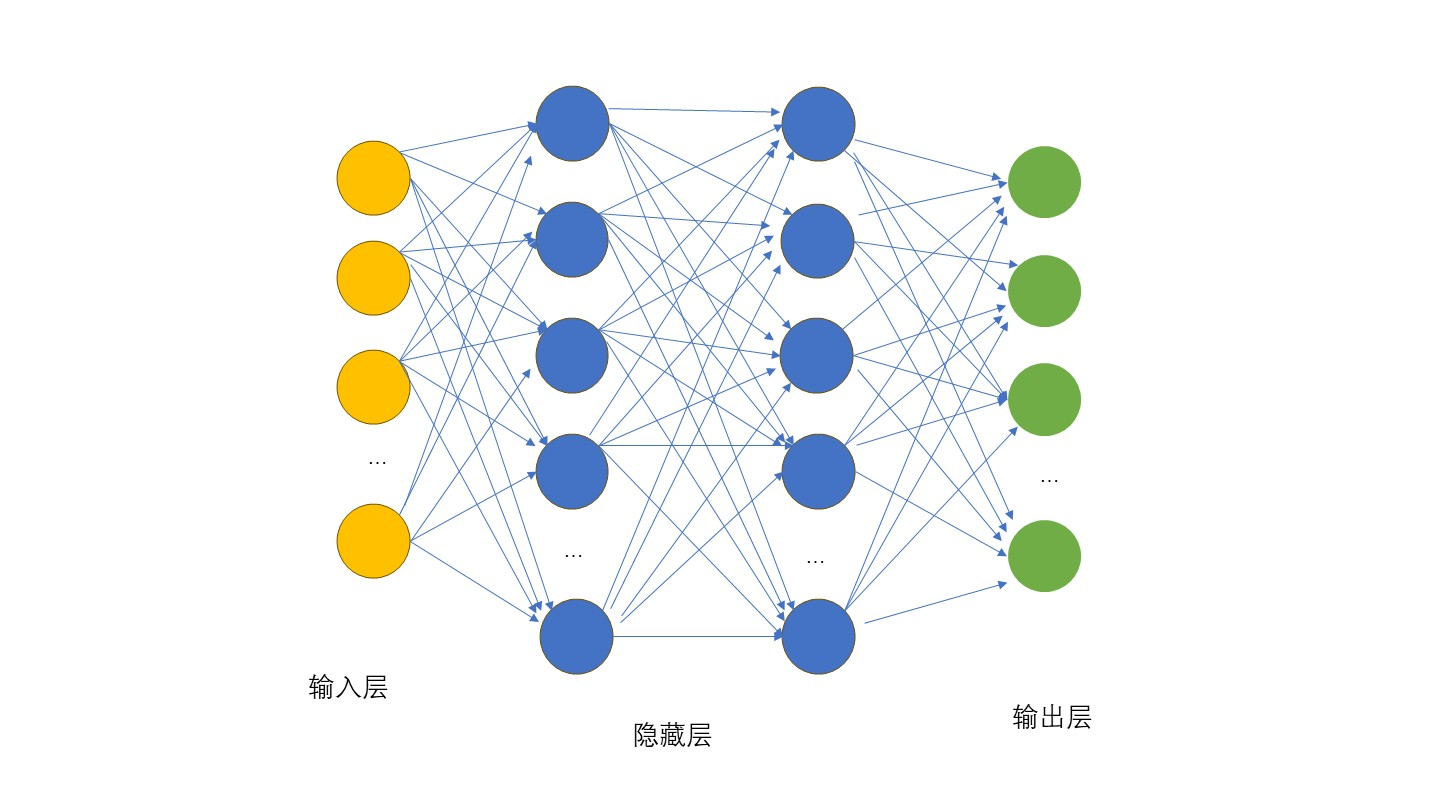
\includegraphics[width=\linewidth]{深度神经网络结构.jpeg}
	\caption{深度神经网络结构}
	\label{f.example}
\end{figure}

我们可以发现,对于高阶神经网络,权重是归一化的,变分参数也是归一化的。然而,损失函数也代表了相应的误差。一般来说,线性回归问题基于平方误差,平方误差被视为损失函数,解释为:

\[
\text{loss}(Y, \hat{Y}) = \frac{1}{N} \sum_{i=1}^{N} \left( \hat{\mathcal{V}}_i - \mathcal{V}_i \right)^2
\]

我们通过研究可以发现,在上述公式中,训练样本数为N,预测值为$\hat{Y}$,实际值为$Y_(i)$。在训练过程中,输入数据可以来回传递以获得所有层的输出数据。这代表了分层网络中神经元的误差。在深度神经网络的训练过程中,反向传播算法扮演着至关重要的角色。一旦通过前向传播获得了各层的输出,就可以利用反向传播来计算每一层神经元的误差,从而进一步计算关于权重和偏置参数的梯度。

\subsection{卷积神经网络}

研究发现,在CNN里,卷积提取图像局部特征,能降低特征图维度,减少特征数量与网络大小,知识库也有所改善,其在网络中采用权重分配方法,能减少参数数量,增加模型泛化效率,提高模型学习效率,卷积神经网络的运用,提升了深度学习在成像任务中的表现,该模型可处理大规模图像数据。计算机视觉领域取得进步且发展较快。
\begin{figure}[hbt]
	\centering
	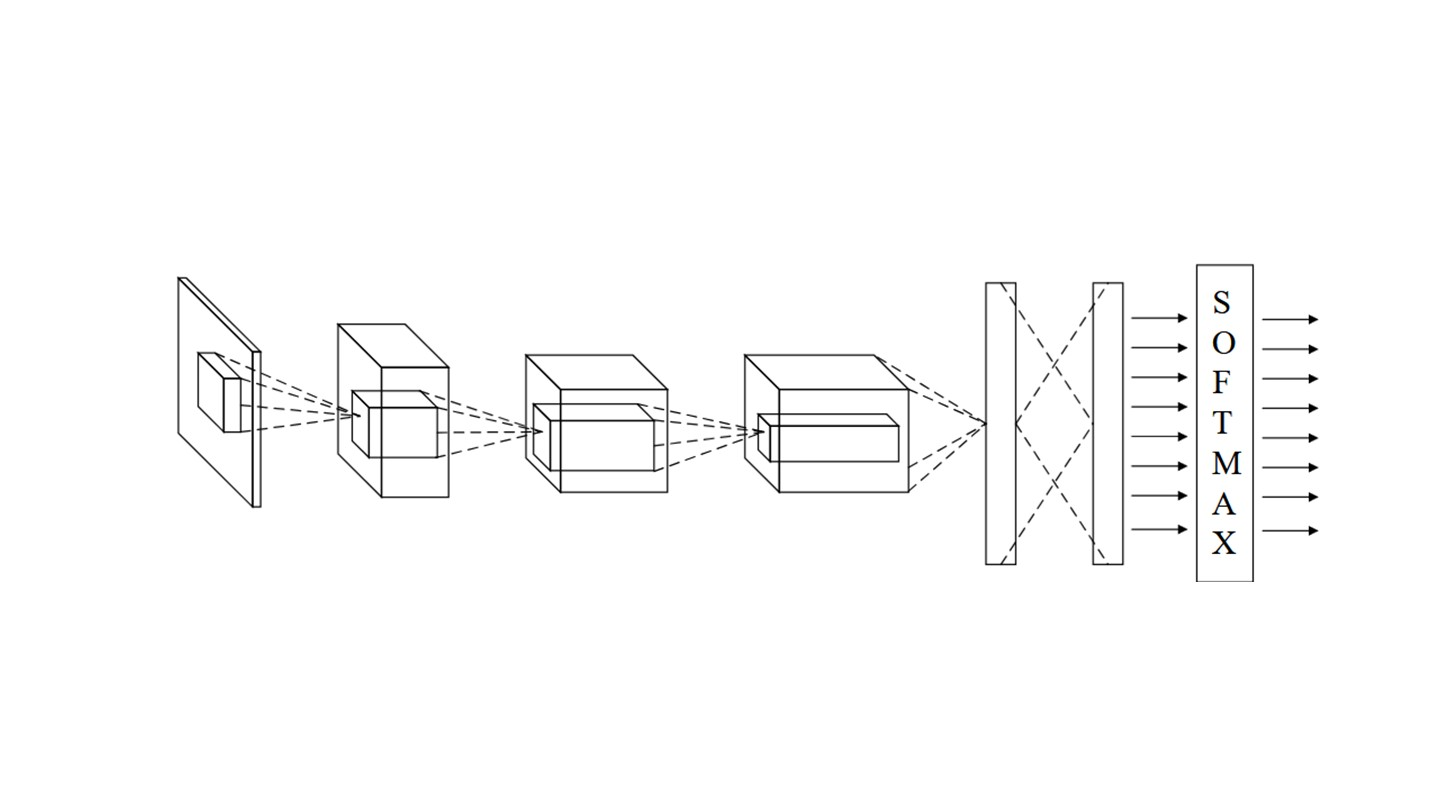
\includegraphics[width=\linewidth]{图像分类卷积神经网络结构示意图.jpeg}
	\caption{图像分类卷积神经网络结构示意图}
	\label{f.example}
\end{figure}

借助观察图2-5可看出其呈现了卷积神经网络的基本结构,卷积神经网络是由多个卷积层以及池化层构成的,这对于输入图像的特征提取以及降维起着十分关键的作用,降低卷积特征图的维度可减少参数数量并且降低计算复杂度,还可以保留图像的关键特征。

经过一系列折叠和汇总操作之后,特征图会被传送到全连接层,此层会组合每个特征图里的特征信息,并且运用非线性函数对其展开操作,以此来捕获特征之间的复杂交互。全连接层的输出会被送至Softmax层,Softmax层运用似然法对结果给予处理,得到各个类的概率分布,以此深入知晓输入图像的分类情况。卷积神经网络结构有强大的特征提取和分类能力,在图像分析、目标检测等任务里可收获优异的效果,在训练进程中,反向传播算法可让网络自动学习特征的最佳表示,对图像展开准确的分类。在卷积神经网络中,常见的输入信号是RGB图像,其中每个像素包含来自红色、绿色和蓝色这三个通道的信息。

例如,VGG-16模型\cite{simonyan2014very}使用的输入数据是 224×224×3 的 RGB 图像。输入数据一旦送入卷积神经网络,就必须经过多层卷积和池化来降低其维度。我们可以发现,在这个例子中,卷积层由两条路径组成:一条是具有多层的卷积层,另一条是最大池化层。一般情况下每个卷积层的卷积核大小为3*3,其经过一个大的合并层进行特征提取,减少特征图尺寸。我们发现,通过执行这些操作并允许网络从输入图像中提取局部重要特征。在卷积过程中,每个卷积核对输入图像进行加权和局部空间的组合,得到神经元的输入。为了显著提高交换网络的非线性能力,我们应该考虑采用更高的输入值作为非线性激活函数。而我们可以发现在现在的各种不同的输入值中,ReLU激活函数被广泛的被人们所使用使用。我们通过上述的行为,我们就可以得到功能图所有区域的输出值。聚合方法采用2×2的最大聚合,即选取每个局部2×2区域内出现的最大值,在保留重要性的前提下,显著降低了数据对象的维度。

\begin{figure}[hbt]
	\centering
	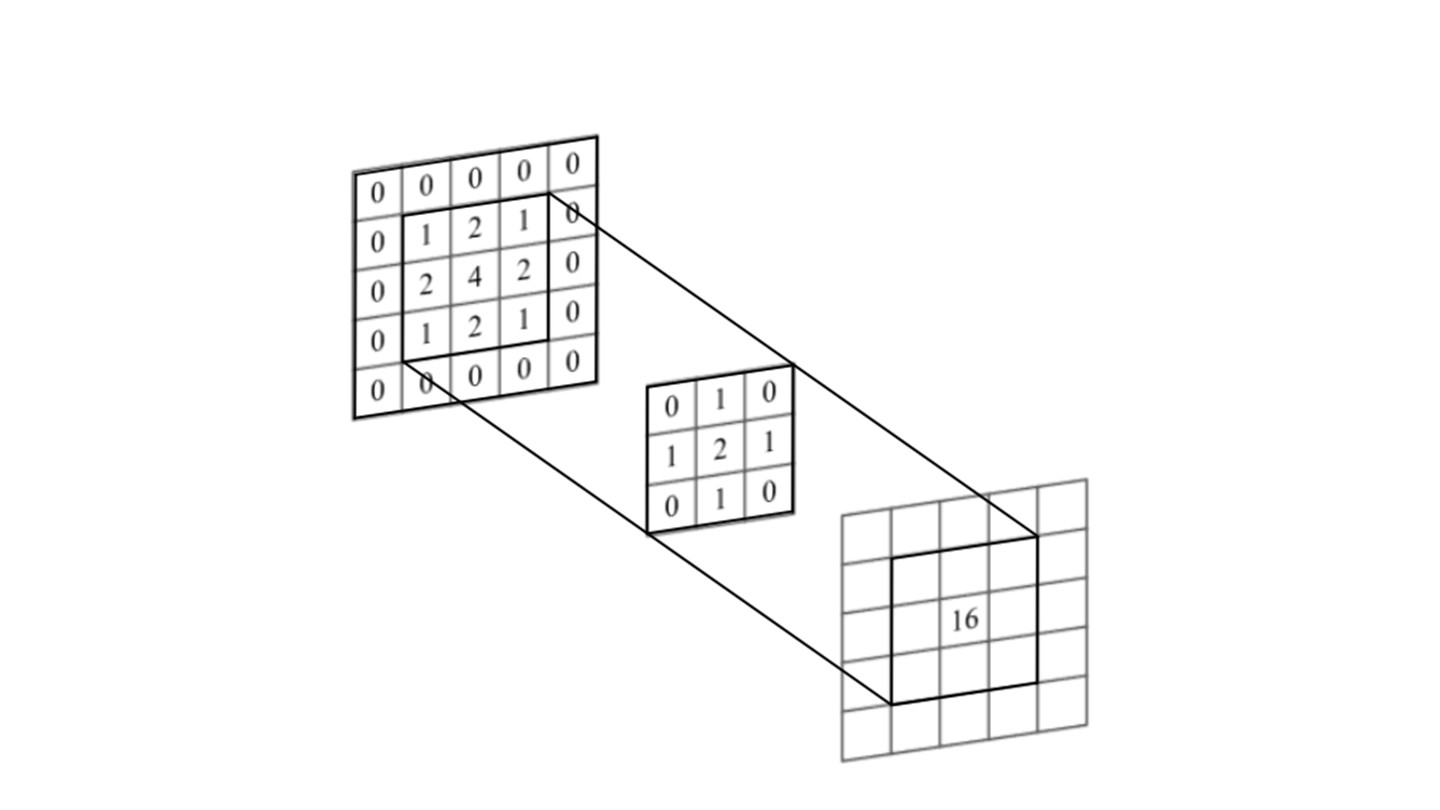
\includegraphics[width=\linewidth]{卷积计算示意图.jpeg}
	\caption{卷积计算示意图}
	\label{f.example}
\end{figure}

我们可以通过现有的研究发现,在 2016 年,国内学者何凯明总结出 ResNet 残差网络\cite{he2016deep},在这个残差网络之中,通过将残差单位加入进
来,不使用其它参数时,可以实现前向反馈神经网络训练。这一单元结构具体见下图2-7。

\begin{figure}[hbt]
	\centering
	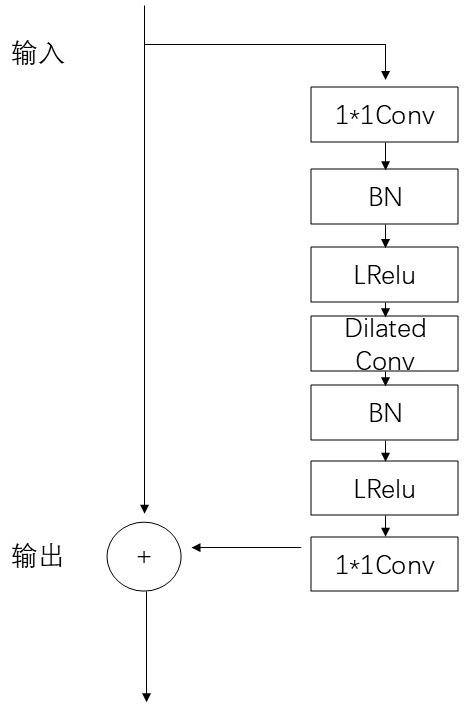
\includegraphics[width=\linewidth]{残差单元.jpeg}
	\caption{残差单元}
	\label{f.example}
\end{figure}

可发现,在执行语义分割之类任务时,卷积神经网络要处理大量像素级数据,这致使网络变得复杂且层次深,尽管这些深度学习方法能给出更好性能与准确结果,可在训练时间及估计方面会产生很大开销,在实时应用以及资源受限环境里,像移动设备或者嵌入式系统,深度神经网络设计要格外留意网络复杂性与计算约束。大型网络无法在这些设备上运行,也契合不了实际需求,在构建深度神经网络过程中,除选择合适规模网络外,还得考虑网络深度,恰当的卷积神经网络深度可在维持效率时,减少间隙数量与计算复杂度,提升卷积神经网络的效率与效果,这需要网格修剪、参数共享和模型压缩等技术来减小网格尺寸且不牺牲性能。

\subsection{循环神经网络}

我们通过研究可以发现,循环神经网络 (RNN)\cite{zaremba2014recurrent}可用于避免在某些会话中运行这些任务时出现非目标计算。它主要由多层循环神经网络组成,如下图2-8所示。我们可以通过求解连续序列中的单元,从而得到一个线性神经网络的结构。数据从前向后流动,单元运行后得到的结果用作下一个单元的输入。线性迭代操作按此顺序执行,结构如图2-8所示。

\begin{figure}[hbt]
	\centering
	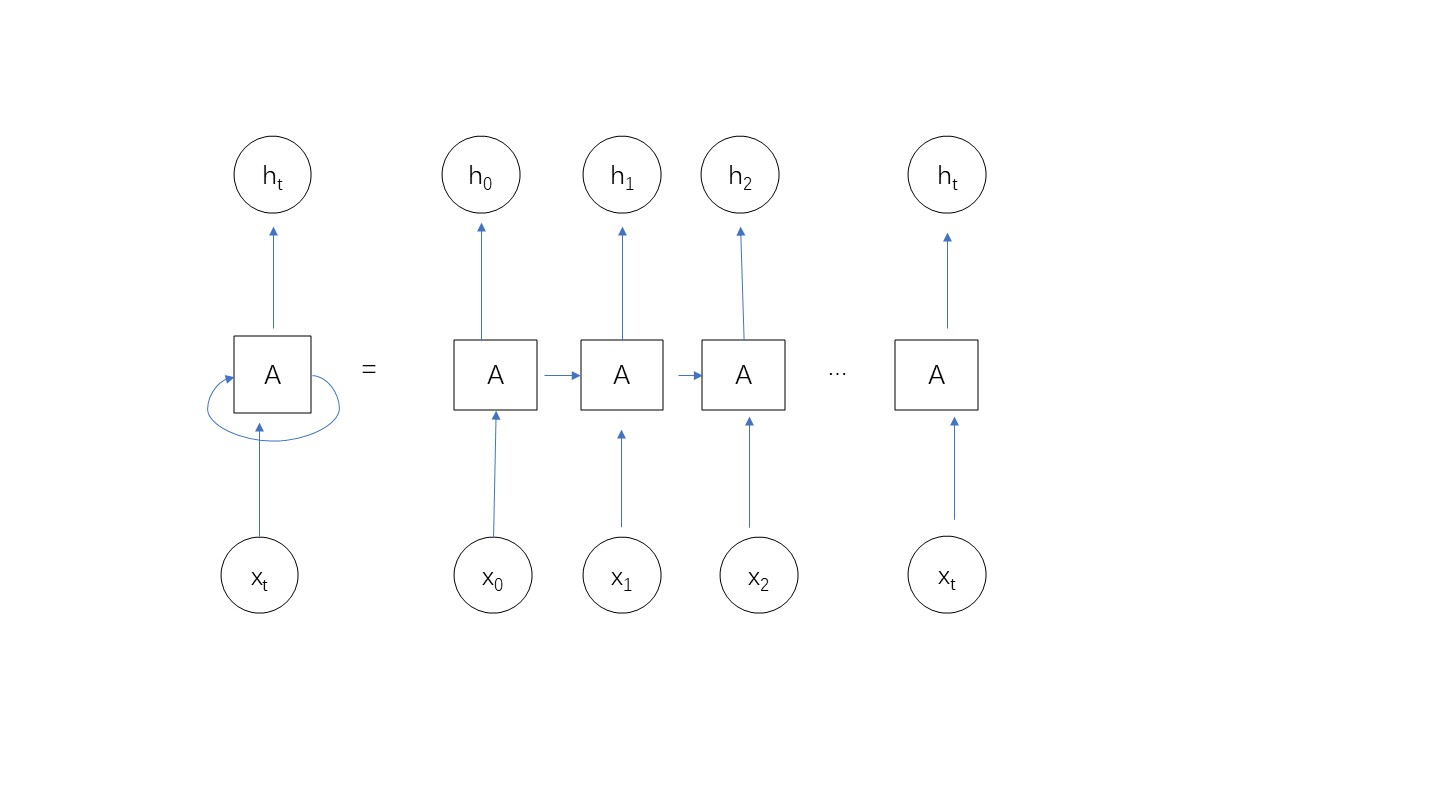
\includegraphics[width=\linewidth]{基础循环神经网络单元.jpeg}
	\caption{基础循环神经网络单元}
	\label{f.example}
\end{figure}

我们可以发现,在循环神经网络的实际实现中,也会出现一些难以有效避免的问题。例如,连接数量的不断增加会导致神经网络的增长,并且这种神经网络的增长无法得到有效的抑制。因此,它在深度联想学习中的作用尚未完全了解。 LSTM\cite{hochreiter1997long}的出现为解决这一问题提供了新的思路。它由三部分组成:输入阀、输出阀和忘记阀。这三个门的加入,使得我们可以忘记不需要记住的信息,保留需要记住的信息,有效地解决了信息长期保留的问题。长短时记忆网络结构如图2-9所示。

\begin{figure}[hbt]
	\centering
	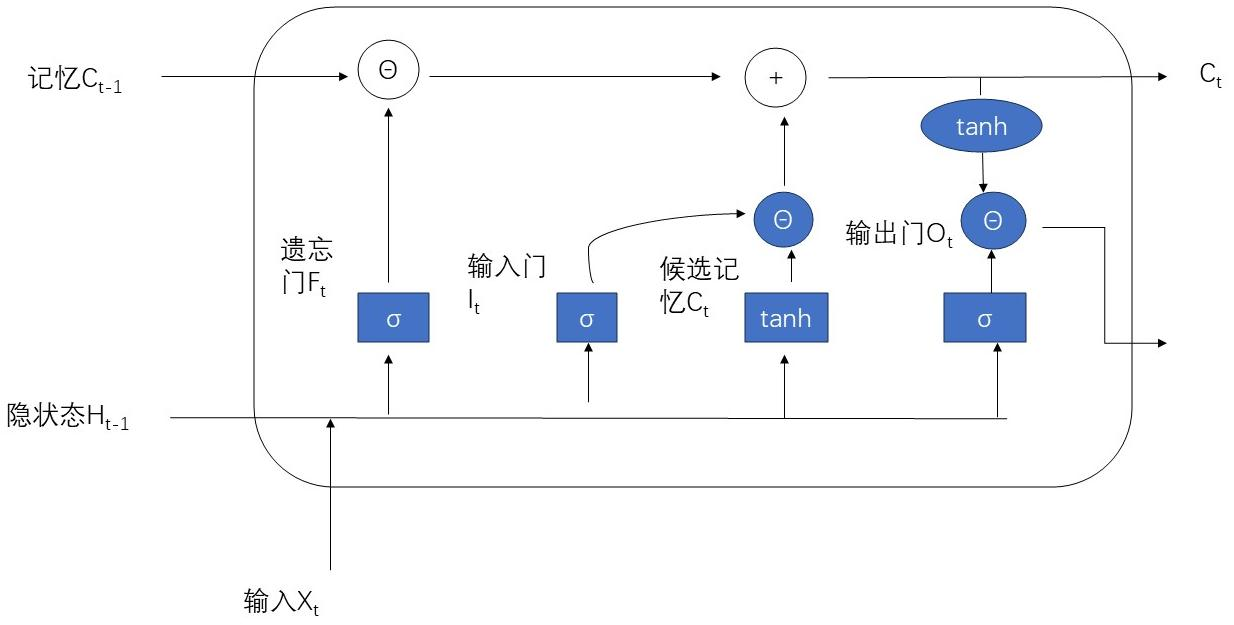
\includegraphics[width=\linewidth]{长短时记忆网络.jpeg}
	\caption{长短时记忆网络}
	\label{f.example}
\end{figure}


